\documentclass[a4paper]{article}

%% Language and font encodings
\usepackage[english]{babel}
\usepackage[utf8x]{inputenc}
\usepackage[T1]{fontenc}

%% Sets page size and margins
\usepackage[a4paper,top=3cm,bottom=2cm,left=3cm,right=3cm,marginparwidth=1.75cm]{geometry}

%% Useful packages
\usepackage{amsmath}
\usepackage{graphicx}
\usepackage[colorinlistoftodos]{todonotes}
\usepackage[colorlinks=true, allcolors=blue]{hyperref}

\title{Reporte de Actividad 5\\Preparando datos con ayuda de Emacs}
\author{Michelle Contreras Cossio}
\date{6 Marzo del 2018}
\begin{document}
\maketitle

\section{Introducción}

En esta actividad, de nuevo se trabajó con la base de datos atmosféricos de la Universidad de Wyoming, utilizando la misma estación en el Aeropuerto Internacional de Adelaida, Australia. Sin embargo, se dió un enfoque bastante diferente. \\

El objetivo de esta práctica fue comprender mejor el uso de Emacs para editar archivos, automatizando así un proceso que, al trabajar con archivos muy grandes, nos podría tomar mucho tiempo. Estos datos, utilizados de nuevo de un año completo, se editaron en Emacs y también con un poco de ayuda del bash, para trabajar únicamente información de las variables CAPE y PW, explicadas en la siguiente sección, y posteriormente se trabajó con estos archivos jupyter. 

\section{Descripción de los conceptos físicos: CAPE y PW}

Durante esta práctica se utilizan datos de las variables "CAPE" y "PW" de la base de datos atmosféricos de la Universidad de Wyoming, durante esta sección se van a definir para poder entender los datos y gráficas que se analizarán.\\

CAPE, por sus siglas en inglés, significa Convective Available Potential Energy, Energía Potencial Convectiva Disponible. Es la cantidad de energía que una parcela de aire tendría si se levantara cierta distancia, verticalmente. Es un indicador de inestabilidad atmosférica y es muy importante al momento de predecir catástrofes atmosféricas, como son tormentas, tornados, granizo, remolinos, etc.\\

PW, por sus siglas en inglés, Precipitable Water, es decir Agua Precipitable, es la cantidad de agua, expresada como altura o masa, que se obtendría si todo el vapor de agua contenido en una columna específica de la atmósfera, se condensara y precipitara. Se mide en milímetros o pulgadas. 

\section{Descripción del proceso de limpieza y preparación de los datos}

En esta sección se explica el proceso que se llevó a cabo para crear los archivos ingresados a pandas. 

\begin{enumerate}
\item Primeramente, se inició tomando el archivo de sondeos.txt creado en la actividad anterior y copiándolo a nuestra nueva carpeta de Actividad5. 
\item Posteriormente, se realizó un script, similar al utilizando en la Actividad 4 para crear el df2017. Pero este nos permitía quedarnos únicamente con los datos de la fecha, CAPE y Precipitable Water, para 00Z y 12Z. \\

\begin{figure}[h!]
  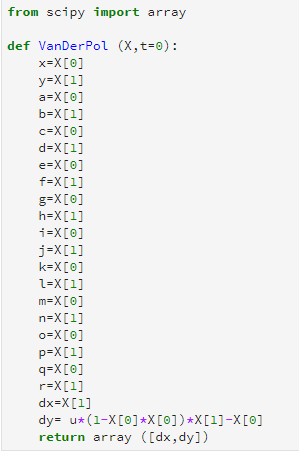
\includegraphics[width=10cm]{1.png}
  \centering
  \label{fig:1}
\end{figure}

\item Una vez corrido el script, se creó un solo archivo llamado df2017CAPE\_PW.csv.

\begin{figure}[h!]
  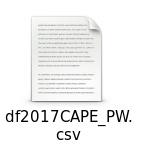
\includegraphics[width=2cm]{2.png}
  \centering
  \label{fig:2}
\end{figure}
\item Este archivo se corrió con emacs, con lo que se pudo observar que contenía información innecesaria, ya que el objetivo era tener un archivo como el siguiente:

\begin{figure}[h!]
  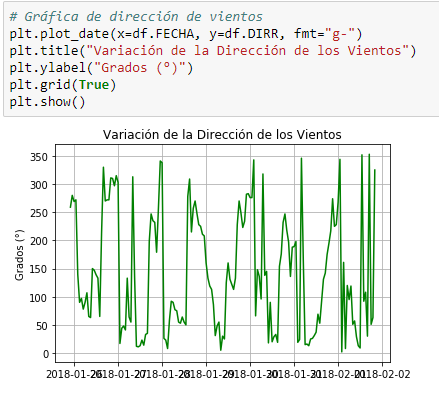
\includegraphics[width=4cm]{3.png}
  \centering
  \label{fig:3}
\end{figure}

Donde la primera columna representara la fecha, la segunda la variable CAPE y la tercera PW. 
\item Para ello, se hizo uso de comandos en emacs. Primero se utilizó el comanto ctrl\textbf{+ }tecla de espacio, que nos permite seleccionar cierta parte del código y, moviendo con las flechas, se seleccionó la parte de código que se deseaba eliminar.
\begin{figure}[h!]
  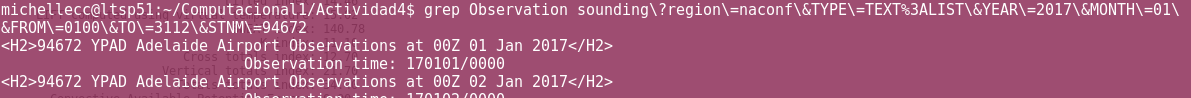
\includegraphics[width=7cm]{4.png}
  \centering
  \label{fig:4}
\end{figure}
\item Posteriormente se utilizó el comando ctrl\textbf{+}w, que borra esa parte seleccionada pero la manda a la memoria. Y se recuperó, en el mismo lugar donde estaba, con ctrl\textbf{+}y, que vacía en el lugar indicado la memoria.
\item Se utilizó el comando esc\textbf{+}<, que nos llevó al inicio del documento. 
\item El comando esc\textbf{+}\% nos permitió abrir el Query replace, comando que nos permite remplazar alguna cadena de código por otra. 
\begin{figure}[h!]
  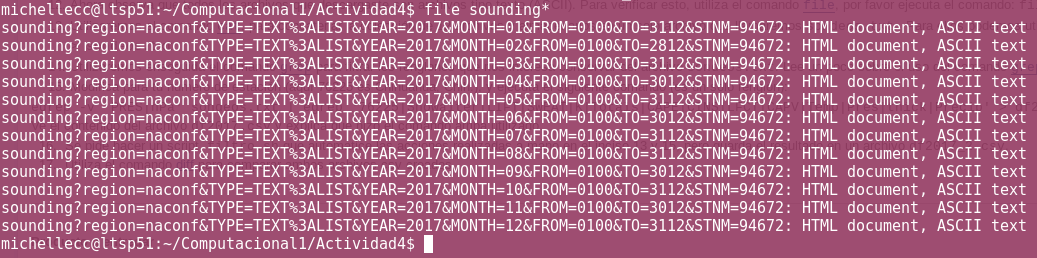
\includegraphics[width=7cm]{5.png}
  \centering
  \label{fig:5}
\end{figure}
\item En el Query replace vaciamos la memoria con el ctrl+y, que es la cadena que queremos reemplazar en el código y damos enter. Después, nos pregunta por cual otra cadena la queremos reemplazar, en el primer caso, sólo se buscaba eliminar esa parte del código, por lo que se reemplazo con nada. Posterior a eso nos marca las partes del código que se van a reemplazar y damos aceptar con el símbolo !. 
\begin{figure}[h!]
  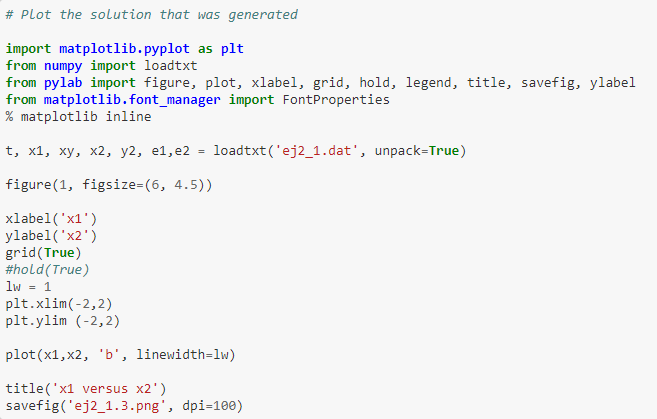
\includegraphics[width=7cm]{6.png}
  \centering
  \label{fig:6}
\end{figure}
\begin{figure}[h!]
  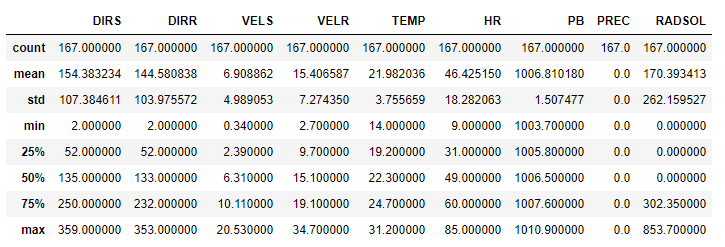
\includegraphics[width=7cm]{7.png}
  \centering
  \label{fig:7}
\end{figure}

\clearpage
\item Así, se eliminó una cadena de código que se repetía una vez para cada uno de los días. 
\begin{figure}[h!]
  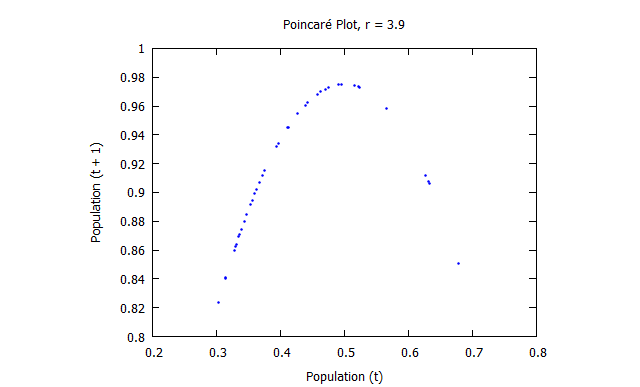
\includegraphics[width=6cm]{8.png}
  \centering
  \label{fig:8}
\end{figure}
\item El proceso realizado de del paso 5 al 10 se repitió para cada una de las cadenas que se quería eliminar o reemplazar, ya fuera por una coma o, en el caso de los meses, se reemplazaron por números.
\item Finalmente, se obtuvo un archivo con renglones de la siguiente manera: \begin{figure}[h!]
  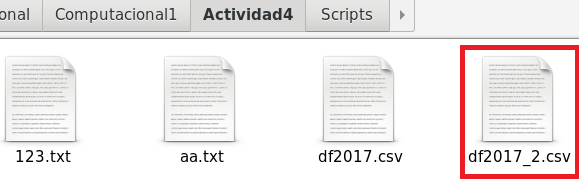
\includegraphics[width=4cm]{9.png}
  \centering
  \label{fig:9}
\end{figure}
\item Como el objetivo era tener dos archivos, uno con los datos del 00Z y otro del 12Z, se utilizaron los siguientes comandos, con grep, lo cual separó el archivo  df2017CAPE\_PW.csv, en dos archivos: df2017CAPE\_PW\_00Z.csv y df2017CAPE\_PW\_12Z.csv. 
\begin{figure}[h!]
  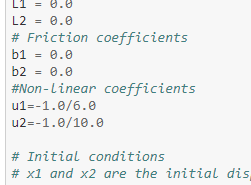
\includegraphics[width=12cm]{10.png}
  \centering
  \label{fig:10}
\end{figure}

\begin{figure}[h!]
  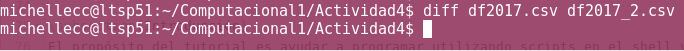
\includegraphics[width=4cm]{11.png}
  \centering
  \label{fig:11}
\end{figure}
\item Los archivos creados tenían al inicio de cada renglón 00Z o 12Z, respectivamente, por lo que utilizando los mismos comando del paso 5 al 10, se eliminaron, para finalmente lograr dos archivos con la misma estructura que el mostrado en el paso 4, para después poder trabajar con los datos en pandas. 
\end{enumerate}


\clearpage
\section{Análisis de datos utilizando Pandas}

En esta sección se muestra como se trabajaron los datos, anteriormente limpiados, para poder realizar gráficas para una mejor visualización y análisis de estos.

\begin{enumerate}
\item Primeramente, y como de costumbre, se cargaron las bibliotecas con las que se trabajó, los procesos posteriores se realizaron para cada uno de los dos archivos creados en la sección anterior.
\begin{figure}[h!]
  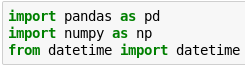
\includegraphics[width=3cm]{A1.png}
  \centering
  \label{fig:A1}
\end{figure}
\item Posteriormente, se leyeron los datos, se asignó nombre a cada columna y se le dió formato de número a la columna CAPE. 
\begin{figure}[h!]
  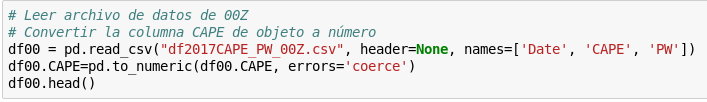
\includegraphics[width=10cm]{A2.png}
  \centering
  \label{fig:A2}
\end{figure}
\item Se creó una nueva columna, con formato de fecha. 
\begin{figure}[h!]
  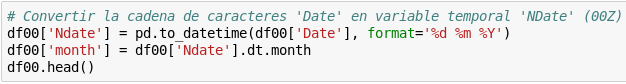
\includegraphics[width=10cm]{A3.png}
  \centering
  \label{fig:A3}
\end{figure}
\item Haciendo uso de la biblioteca seaborn y matplotlib realizaron las gráficas de boxplot, por mes, la primera del CAPE y la segunda del PW.
\begin{figure}[h!]
  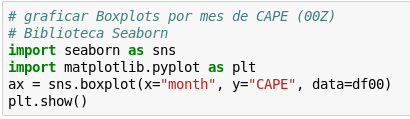
\includegraphics[width=5.5cm]{A4.png}
  \centering
  \label{fig:A4}
\end{figure}
\begin{figure}[h!]
  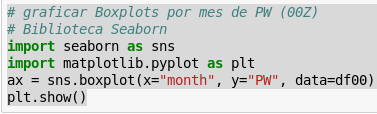
\includegraphics[width=5cm]{A5.png}
  \centering
  \label{fig:A5}
\end{figure}
\item Utilizando la misma biblioteca, seaborn, se creó el jointplot, que compara las variables CAPE y PW. 
\begin{figure}[h!]
  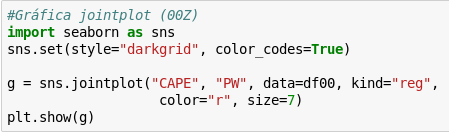
\includegraphics[width=6cm]{A6.png}
  \centering
  \label{fig:A6}
\end{figure}
\item Finalmente, se creó la gráfica de lmplot de PW vs CAPE, donde crea un modelo de regresión lineal para cada uno de los meses.
\end{enumerate}
\begin{figure}[h!]
  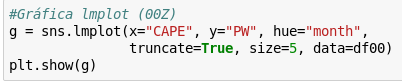
\includegraphics[width=6cm]{A7.png}
  \centering
  \label{fig:A7}
\end{figure}

\section{Resultados del análisis}

Los pasos mostrados en la sección anterior crearon un total de 8 gráficas, analizadas a continuación: 

\begin{itemize}
\item \textbf{Archivo de datos df2017CAPE\_PW\_00Z.csv: }
Debido a la zona horaria en la que se encuentra, los sondeos en 00Z se realizaron a las 12pm. 
\begin{itemize}
\item \textbf{Boxplot:} \\
\begin{itemize}
\item CAPE: 
\begin{figure}[h!]
  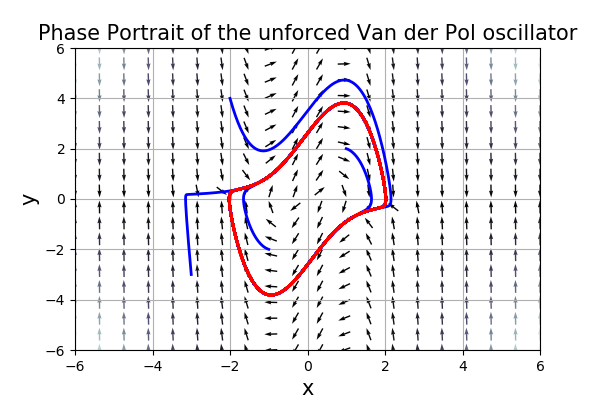
\includegraphics[width=10cm]{Graf1.png}
  \centering
  \label{fig:G1}
\end{figure}

Este diagrama de caja muestra que en todo el año, a las 12 pm, la variable CAPE esta alrededor del cero, aunque existen valores muy fuera del rango, son pocos.\\

\item PW: \\
\begin{figure}[h!]
  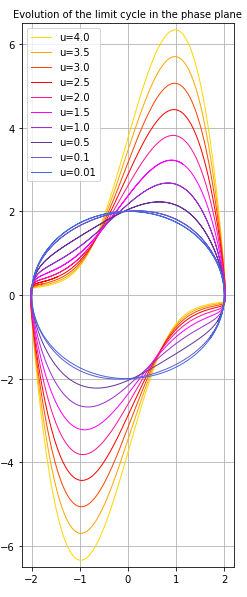
\includegraphics[width=10cm]{Graf2.png}
  \centering
  \label{fig:G2}
\end{figure}

Por su parte, este diagrama de caja del agua precipitable, muestra que la media en general esta alrededor de los 15 y 25 mm. Sin embargo, se nota un poco la variación, donde de diciembre a febrero, es decir, el verano en Australia, este índice es más alto que de junio a agosto, donde es invierno. 
\end{itemize}

\clearpage

\item \textbf{Jointplot}:\\
\begin{figure}[h!]
  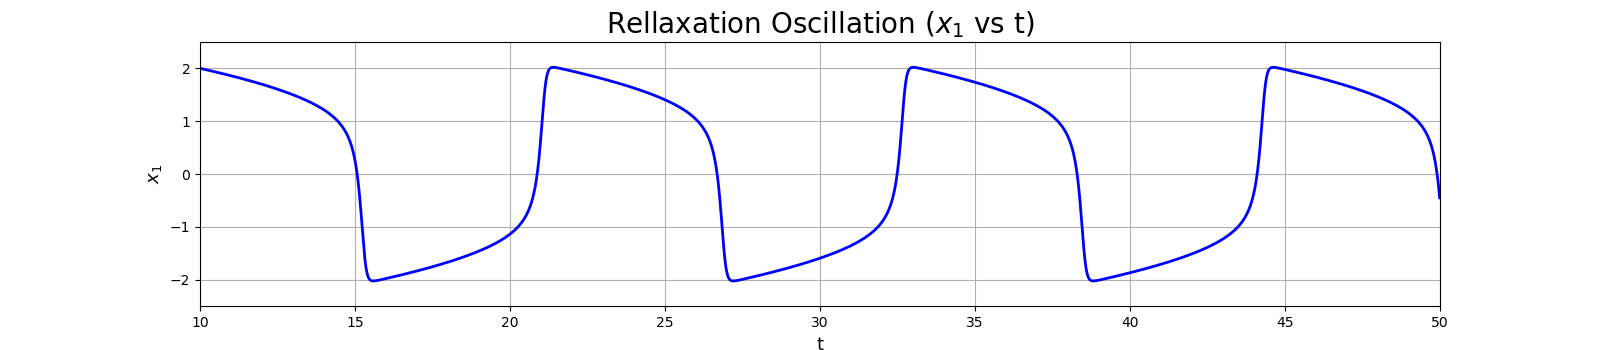
\includegraphics[width=10cm]{Graf3.png}
  \centering
  \label{fig:G3}
\end{figure}

Esta gráfica de PW vs CAPE nos muestra el coeficiente de correlación de Pearson, donde podemos observar que las variables si estan ligadas linealmente y positivamente, ya que este es igual a 0.2. La gráfica además muestra la recta que mejor se aproxima, así como la distribución de cada una de las variables. Podemos observar, que la variable CAPE se distribuye en su mayoría alrededor del 0 y la variable PW alrededor del 20.\\

\item\textbf{ Lmplot:}\\
\begin{figure}[h!]
  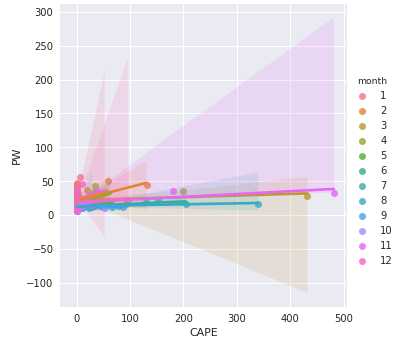
\includegraphics[width=10cm]{Graf4.png}
  \centering
  \label{fig:G4}
\end{figure}
\end{itemize}

El Lmplot grafíca PW contra CAPE, pero de cada mes, para así ver como varían ambas, según cambian las estaciones del año. Para cada mes creó una recta de regresión lineal, se puede observar que los meses donde el CAPE es más alto, el PW es más bajo.

\item \textbf{Archivo de datos df2017CAPE\_PW\_12Z.csv: }
Debido a la zona horaria en la que se encuentra, los sondeos e 12 e realizaron a las 12am.
\begin{itemize}
\item \textbf{Boxplot:}
\begin{itemize}
\item CAPE: 
\begin{figure}[h!]
  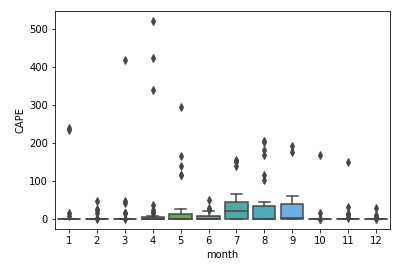
\includegraphics[width=10cm]{Graf5.png}
  \centering
  \label{fig:G5}
\end{figure}

Podemos observar que a las 12 am, existe una pequeña variación que con la gráfica de las 12 pm. El CAPE ya no se encuentra tan cercano al cero, en los meses de invierno, este aumenta. \\

\item PW: \\
\begin{figure}[h!]
  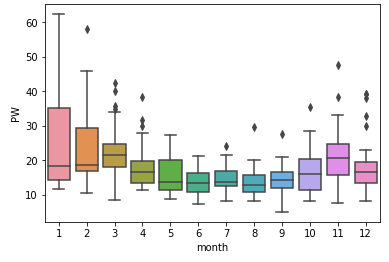
\includegraphics[width=10cm]{Graf6.png}
  \centering
  \label{fig:G6}
\end{figure}

Este boxplot si es bastante similar al de las 12 pm, la variación existe en el tamaño del rango intercuartílico, que en este caso se ve un poco más extenso. 
\end{itemize}

\clearpage

\item \textbf{Jointplot:}\\
\begin{figure}[h!]
  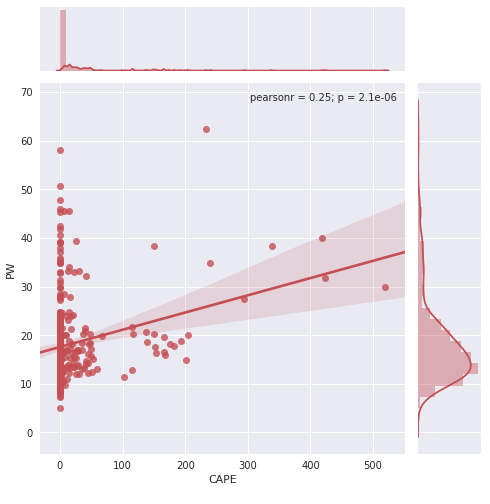
\includegraphics[width=10cm]{Graf7.png}
  \centering
  \label{fig:G7}  
\end{figure}

Esta gráfica muestra una mayor correlación lineal, con un tamaño de 0.25 y las distribuciones se encuentran similares a las de las 12 pm, alrededor de los mismo valores. \\

\item \textbf{Lmplot:}\\
\begin{figure}[h!]
  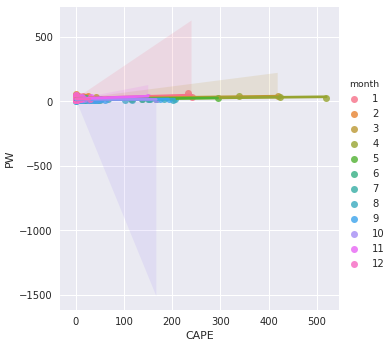
\includegraphics[width=10cm]{Graf8.png}
  \centering
  \label{fig:G8}
\end{figure}

Por último, esta gráfica difiere un poco con la de las 12 pm, ya que muestra que el PW no varió mucho entre los meses. 

\end{itemize}
\end{itemize}


\section{Conclusiones}

Como conclusión, me gustaría agregar que el objetivo fue cumplido, ya que se pudo realizar una limpia de datos bastante extensos, como se mencionó, eran de un año; tal y como se requerían, de una manera muy rápida, se logró en menos de 40 minutos. Si estos datos se hubieran ingresado en pandas antes de ser editados y limpiados, el proceso probablemente hubiera sido más largo y tedioso, con muchos tropiezos e incluso sin haber podido llegar a lo que se requería. \\

La moraleja que me queda tras esto es que subestime mucho el uso que se le podía dar a Emacs, sobre todo porque nunca había trabajado en un procesamiento de datos con una cantidad grande de estos, lo comparaba mucho con el Bloc de Notas en Windows, pero veo que permite realizar procesos de una manera más automática y nos permite "ser flojos".

\section{Bibliografía}
\begin{itemize}
\item Convective available potential energy (2018). Consultado: 2 de Marzo del 2018, de Wikipedia. Sitio web: https://en.wikipedia.org/wiki/Convective\_available\_potential\_energy
\item Precipitable Water (2018). Consultado: 2 de Marzo del 2018, de Wikipedia. Sitio web:\\ https://en.wikipedia.org/wiki/Precipitable\_water
\item Agua precipitable. Consultado: 2 de Marzo del 2018, de Agua Market. Sitio web: \\ http://www.aguamarket.com/diccionario/terminos.asp?Id=4550
\end{itemize}

\section{Apéndice}

\begin{enumerate}
\item ¿Cómo se te hizo esta actividad? ¿Compleja, Difícil, Sencilla?

Se me hizo bastante sencilla.

\item ¿Qué te llamó más la atención?

El uso de emacs, nunca me había dado la oportunidad de usarlo o aprender sus comandos y es bastante útil.

\item ¿Qué parte fue la que menos te interesó hacer?

No hubo nada que me desinteresara, hubo cosas neutrales, pero no con desinterés o que no me gustaran.

\item ¿Cómo mejorarías esta actividad? ¿Qué le faltó? ¿Qué sobró?

Me hubiera gustado hacer más uso de pandas, que nos pidiera algo que no viniera en el ejemplo.

\item ¿Hasta este punto, que te parece el uso de Jupyter para programar en Python? 

Me ha gustado mucho y me parece sencillo, hasta el momento.

\end{enumerate}

\end{document}